\section{Композиции алгоритмов. Градиентный бустинг}

При решении сложных задач классификации, регрессии, прогнозирования часто оказывается, что ни один из алгоритмов не обеспечивает желаемого качества восстановления зависимости. В таких случаях имеет смысл строить композиции алгоритмов, в которых ошибки отдельных алгоритмов взаимно компенсируются. Наиболее известные примеры композиций — простое и взвешенное голосование. 

\subsection{Композиция алгоритмов}
Введем множество объектов $X$ и множество ответо $Y$. Наряду с этими множествами, введем вспомогательное множество $R$, называемое пространством оценок. Рассматриваются алгоритмы, имеющие вид суперпозиции $a(x)=C(b(x))$, где функция $b: X \to R$ называется алгоритмическим оператором, функция $C: R \to Y$ - решающее правило. 

Многие алгоритмы классификации имеют именно такую структуру: сначала вычисляются оценки принадлежности объекта классам, затем решающее правило переводит эти оценки в номер класса. Значением оценки $b(x)$ может быть вероятность принадлежности объекта x классу, расстояние от объекта до разделяющей поверхности, степень уверенности классификации и т.п.

Введем полное определение классификатора, на основе модели композиции. Композицией $T$ алгоритмов $a_t(x)= C(b_t(x)), t=1,\dotsc,T$ называется суперпозиция алгоритмических операторов $b_t: X \to R$, корректирующей операции  $F: R^T \to R$ и решающего правила $C: R \to Y$:


\begin{equation}
	a(x) = C(F(b_1(x),\dotsc,b_T(x))), x \in X
\end{equation}

Алгоритмы $a_t$, а иногда и операторы $bt$ , называют базовыми алгоритмами. 
Суперпозиции вида $F(b_1,\dotsc, b_T)$ являются отображениями из $X$ в $R$, то есть, опять-таки, алгоритмическими операторами. Это позволяет строить иерархические композиции, применяя определение 1.1 рекурсивно.

Пространство оценок $R$ вводится для того, чтобы расширить множество допустимых корректирующих операций. Можно было бы определить корректирующую операцию и как отображение $F: Y^T \to Y$ , то есть комбинировать непосредственно ответы базовых алгоритмов. Однако в задачах классификации, когда множество $Y$ конечно, число «разумных» корректирующих операций такого вида невелико, что ограничивает возможность оптимизации $F$ под конкретную задачу \todobiography. Если же ком бинировать ответы алгоритмических операторов, то операция $F$ получает на входе оценки принадлежности объекта классам — более точную информацию, не огрублённую решающим правилом.

\subsection{Взвешанное голосование}

Корректирующая операция $F$ может иметь параметры, настраиваемые по обучающей выборке, наряду с параметрами базовых алгоритмов. Например, в линейной комбинации настраиваются веса $at$ базовых алгоритмов:

\begin{equation}
	b(x)=F(b_1(x), \dotsc ,b_T(x)) = \sum_{t=1}^{T} a_tb_t(x),  x \in X,  a_t \in R
\end{equation}

Если веса $a_t$ неотрицательны и нормированы, $\sum_{t=1}^{T} a_t =1$ , то композицию (1.2) называют выпуклой комбинацией базовых алгоритмов. Естественно предполагать, что вес $a_t$ тем больше, чем выше качество базового алгоритма $b_t$.

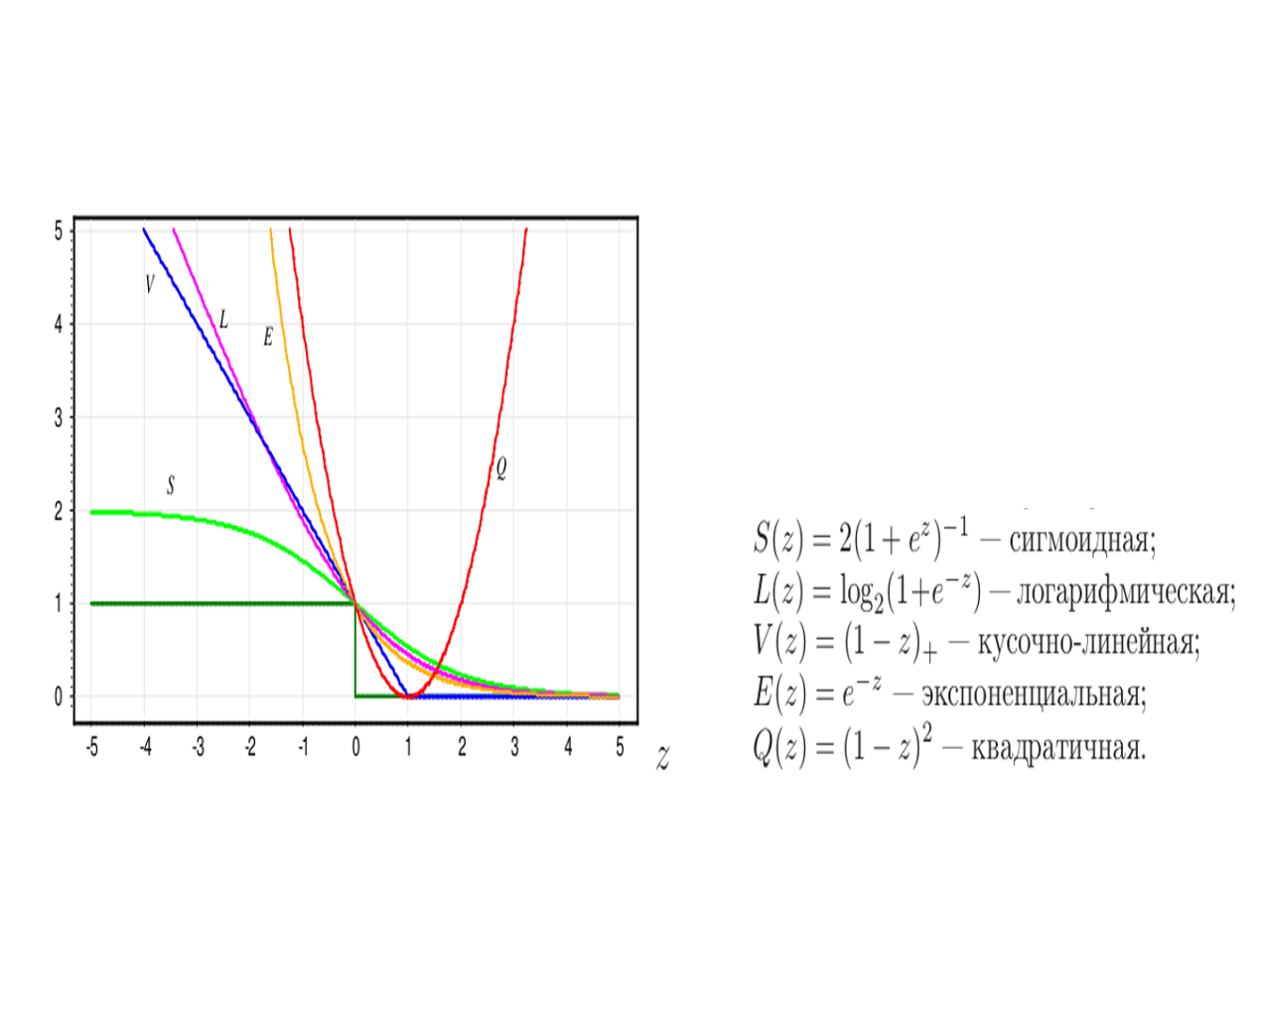
\includegraphics[width=0.9\textwidth]{images/upper_approximations.png}

\subsection{Бустинг}

Построение бустинга лучше всего рассматривать на задаче для двух классов ${-1,1}$, а потом обобщить на общий случай, для множества классов $M$. Пусть есть двух классовая задача $Y={-1,+1}$. Допустим, что решающее правило фиксировано, $C(b) = sign(b)$, базовые алгоритмы возвращают ответы $-1,0,+1$. Ответ $b_t(x) = 0$ означает, что базовый алгоритм $b_t$ отказывается от классификации объекта $x$, и ответ $b_t(x)$ не учитывается в композиции.
Искомая алгоритмическая композиция имеет вид:
\begin{equation}
	a(x)=C(F(b_1(x),\dotsc,b_T(x)))=sign(\sum_{t=1}^{T} a_tb_t(x)), x \in X
\end{equation}

Определим функционал качества композиции как число ошибок, допускаемых
ею на обучающей выборке:
\begin{equation}
	Q_T=\sum_{t=1}^{l} y_i\sum_{t=1}^{T} a_tb_t < 0]
\end{equation}

Напрямую, оптимизировать такой функционал очень сложно, поэтому заменим его на оценку сверху:
\begin{equation}
	Q_T=min_{\beta_m,\gamma_m}\sum_{i=1}^{N}L(y_i,\sum_{m=1}^{M}\beta_m b(x_i;\gamma_m)))
\end{equation}
В качестве функции потерь $L(y_i,f_m(x;\gamma)$ могут выступать функции, приведенные на рисунке 1.
Общий алгоритм бустинга:

\begin{algorithm}
  \caption{Общий алгоритм бустинга}
  \label{overall-boosting-algorithm}
  \begin{enumerate}
  \item Инициализировать переменные $f_0(x)=0$
  \item Для каждого шага $m=1,2 .. M$:
    \begin{enumerate}
      \item Вычисляем $(\beta_m,\gamma_m)=arg \min_{\beta,\gamma} \sum_{i=1}^{N}L(y_i,f_{m-1}(x_i)+\beta b(x_i;\gamma))$
      \item $f_m(x)=f_{m-1}(x)+\beta_m b(x;\gamma_m)$
    \end{enumerate}
  \end{enumerate}
\end{algorithm}



\begin{algorithm}
  \caption{Градиентный бустинг для многоклассовой классификации}
  \label{gradient-boosting-algorithm}
  \begin{enumerate}
  \item Инициализировать переменные $f_0(x)=0, k=1,2,...,K$
  \item Для каждого шага $m=1,2 .. M$:
    \begin{enumerate}
      \item Вычислить:
      \begin{equation}
      	p_k(x)=\frac{e^{f_k(x)}}{\sum_{l=1}^{K}e^{f_l(x)}}, k=1,2,...,K
      \end{equation}
      \item Для k = 1 до K:
      \begin{enumerate}
      	\item $r_{ikm}=y_{ik}-p_k(x_i), i=1,2,...,N$, где $y_{ik}=1$ если $y_i$ принадлежит классу $k$, иначе 0.
      	\item Для множества пар $(x_i,r_ikm)$ построить решающее дерево. С конечными регионами: $R_{jkm}, j=1,2,...,J_m$
      	\item $\gamma_{jkm}=\frac{K-1}{K}\frac{\sum_{x_i\in R_{jkm}}r_{ikm}}{\sum_{x_i\in R_{jkm}}|r_{ikm}|(1-|r_{ikm}|})$
      	\item Обновить $f_{km}=f_{k,m-1}(x)+\sum_{j=1}^{J_m}\gamma_{jkm}I(x\in R_{jkm}$
      \end{enumerate}
    \end{enumerate}
    \item Выход: $f_k=f_{km}(x), k=1,2,...,K$
  \end{enumerate}
\end{algorithm}